\documentclass[12pt,letterpaper]{article}
\usepackage[utf8]{inputenc}
\usepackage[spanish]{babel}
\usepackage{graphicx}
\usepackage[left=2cm,right=2cm,top=2cm,bottom=2cm]{geometry}
\usepackage{graphicx} % figuras
% \usepackage{subfigure} % subfiguras
\usepackage{float} % para usar [H]
\usepackage{amsmath}
%\usepackage{txfonts}
\usepackage{stackrel} 
\usepackage{multirow}
\usepackage{enumerate} % enumerados
\renewcommand{\labelitemi}{$-$}
\renewcommand{\labelitemii}{$\cdot$}
% \author{}
% \title{Caratula}
\begin{document}

% Fancy Header and Footer
% \usepackage{fancyhdr}
% \pagestyle{fancy}
% \cfoot{}
% \rfoot{\thepage}
%

% \usepackage[hidelinks]{hyperref} % CREA HYPERVINCULOS EN INDICE

% \author{}
\title{Caratula}

\begin{titlepage}
\begin{center}
\large{UNERSIDAD PRIVADA DE TACNA}\\
\vspace*{-0.025in}
\begin{figure}[htb]
\begin{center}

\includegraphics[width=8cm]{./Imagenes/logo}
\end{center}
\end{figure}
\vspace*{0.15in}
INGENIERIA DE SISTEMAS  \\

\vspace*{0.5in}
\begin{large}
TITULO:\\
\end{large}

\vspace*{0.1in}
\begin{Large}
\textbf{INFORME DE LABORATORIO No 01} \\
\end{Large}

\vspace*{0.3in}
\begin{Large}
\textbf{CURSO:} \\
\end{Large}

\vspace*{0.1in}
\begin{large}
BASE DE DATOS II\\
\end{large}

\vspace*{0.3in}
\begin{Large}
\textbf{DOCENTE(ING):} \\
\end{Large}

\vspace*{0.1in}
\begin{large}
 Patrick Cuadros Quiroga\\
\end{large}

\vspace*{0.2in}
\vspace*{0.1in}
\begin{large}
Integrantes: \\
\begin{flushleft}


Angelo Brian Quispe Mamani		\hfill	(2015052826) \\

\end{flushleft}
\end{large}
\end{center}

\end{titlepage}


\tableofcontents % INDICE
\thispagestyle{empty} % INDICE SIN NUMERO
\newpage
\setcounter{page}{1} % REINICIAR CONTADOR DE PAGINAS DESPUES DEL INDICE

\section{Actividad No 01 – GitHub} 
GitHub es una importante herramienta para el acceso centralizado a los proyectos gracias a las ventajas que plantea el alojamiento de codigo. En este sentido, el servicio permite que varios participantes trabajen en un mismo proyecto a nivel global y que guarden sus cambios en cualquier momento de forma independiente. A diferencia de otros proveedores de servicios, en lo que respecta a la administracion de software open source, en GitHub el foco de atencion no se situa en el el proyecto como una compilacion de codigo fuente, sino en la posibilidad de hacer uso individualizado de los repositorios(Gestionados con Git). Los usuarios de Github pueden utilizar Git para gestionar, revisar y preparar sus proyectos de software

\begin{itemize}

	\item\textbf {Ventajas e Desventajas}

	Una ventaja importante de GitHub es que el servicio pone a disposici\'on de todos los usuarios repositorios de c\'odigo p\'ublicos y libres sin l\'imites. Sin embargo, el mantenimiento de repositorios privados está sujeto al pago de una suscripción mensual. GitHub también ofrece la posibilidad de crear “organizaciones” que hacen las veces de cuentas regulares a menos que tengas como mínimo una cuenta de usuario de tu propiedad.

A pesar de todo, en algunos casos puede haber ciertas limitaciones en lo relativo a la facilidad de uso y eficiencia de GitHub. En ocasiones surgen complicaciones entre el programa cliente y la compañ\'ia cuando, por ejemplo, un servidor privado opera como host para el código creado. Otra de las razones que motivan la elección de alternativas a GitHub es el empleo de un VCS diferente no soportado por GitHub. Hoy en d\'ia existen diversas alternativas a GitHub, pero en el presente artículo te hablamos de cinco de ellas.
	\begin{center}
	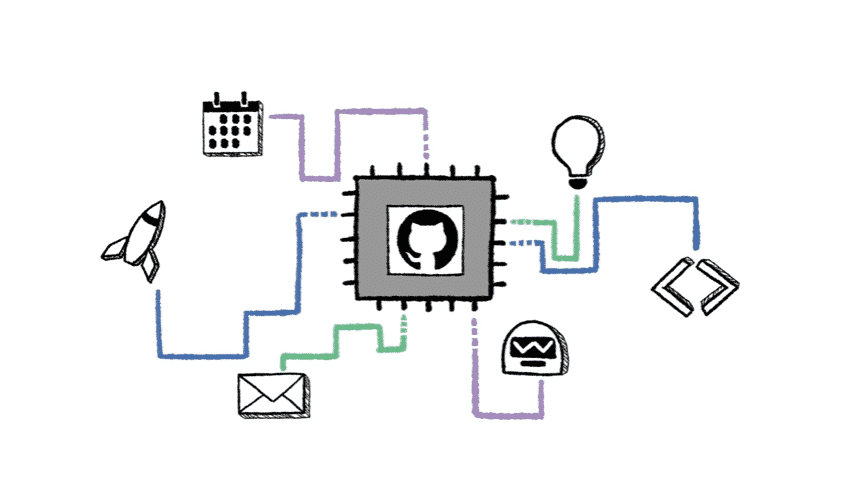
\includegraphics[width=17cm]{./Imagenes/git} 
	\end{center}


\end{itemize} 
\section{Actividad No 02 – GitLab} 
GitLab nació como un sistema de alojamiento de repositorios Git, es decir, un hosting para proyectos gestionados por el sistema de versiones Git. Sin embargo, alrededor de esta herramienta han surgido muchas otras herramientas muy interesantes para programadores y equipos de desarrollo, que envuelven todo el flujo del desarrollo y el despliegue de aplicaciones, test, etc.
\begin{itemize}

	\item Uso

	GitLab es una herramienta basada en Git, que usas de la misma manera que cualquier otra herramienta similar. Generalmente usas Git a través de la línea de comandos, o a través de programas de interfaz gráfica, o del propio editor de código. Toda esa operativa que ya conoces y que hemos explicado en el Manual de Git, no cambia.

Además del hosting remoto para repositorios GitLab ofrece una interfaz web para controlar el repositorio y muchas otras herramientas. Ofrece la posibilidad de examinar el código en cualquiera de sus versiones, realizar acciones relacionadas con el sistema de repositorios como mergear el código de versiones de proyecto o gestionar las "pull request" (que en GitLab se llaman "merge request"), gestionar problemática de tu software diversa, automatizar procesos como el despliegue o la ejecución de pruebas del software, etc. Toda esta operativa la realizas, o configuras, en GitLab por medio de una web.

	

           \item\textbf{ Funcionalidades}
    
	En GitLab podemos gestionar principalmente proyectos, Grupos y Sinppets. Los proyectos son los protagonistas del sistema, básicamente repositorios de software gestionados por GitLab y todo el ecosistema GitLab. Los grupos son básicamente empresas y usuarios. Los snippets por su parte son como pedazos de código que puedes dejar para hacer cualquier cosa.

Como decimos, dentro de los proyectos es donde se aglutinan la mayoría de las funcionalidades que vamos a resumir:

          \textbf {Overview:}
           Es un listado de todo el proyecto, los archivos, los README.md. Es parecido a lo que vemos cuando accedemos a un proyecto con GitHub. Te da el resumen del repositorio, archivos, commits, etc.

Luego tiene dos subsecciones: En Activity del proyecto te ofrece toda la actividad, de una manera estadística. En Cycle Analytics además te ofrece algo muy novedoso, no disponible en otras herramientas. Básicamente informa el tiempo que se tarda en realizar una funcionalidad, desde que tienes la idea hasta que se incorpora al software, de modo que cualquier persona, incluso sin conocimientos de programación, puede saber el tiempo que ocupó el hacer las tareas. Una información muy valiosa que puede ayudar a futuro a estimar mejor el tiempo de trabajo necesario para nuevas funcionalidades. Obviamente, cuantas más issues tengas en el sistema, más datos tendrás para saber el tiempo que necesitas para las próximas tareas.

           \textbf {Repository:}
Dentro de la sección "Repository" tenemos varias opciones diversas que afectan al repositorio del proyecto.

Tenemos "Files", donde se puede navegar por los directorios y archivos, cuyo código podemos ver, e incluso editar los ficheros. Está disponible una visualización por ramas y dispone de utilidades diversas para poder hacer cosas relacionadas con el repositorio remoto, ahorrando la necesidad de lanzar comandos. Tiene un buscador de archivos muy potente.


           \textbf {Issues:}
Este es otra de las grandes utilidades de GitLab, que permite definir cualquier problema que se detecta en el software y darle seguimiento. Seguro que las conocemos porque es una de las partes fundamentales de GitHub y habremos navegado por ellas en decenas de ocasiones.

Básicamente nos permite ver las issues generadas en un proyecto, mantener discusiones sobre ellas, y controlar los flujos de trabajo para su resolución, permitiendo definir las personas que deben resolverla, el tiempo estimado y el usado, la fecha límite, el peso de las tareas, etc.

      

	\begin{center}
	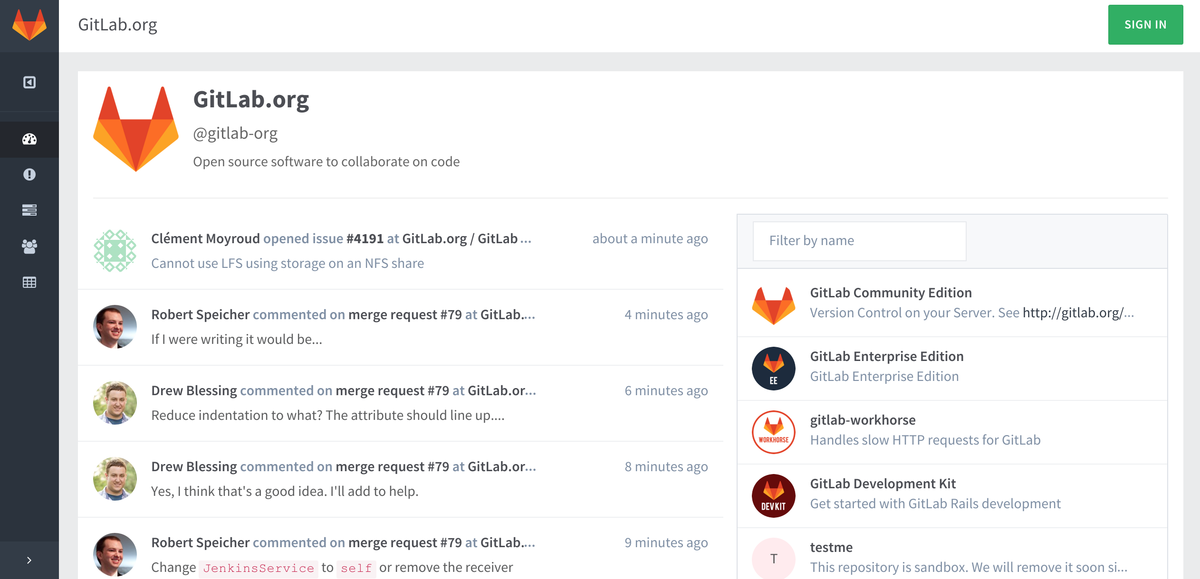
\includegraphics[width=17cm]{./Imagenes/image3} 
	\end{center}


\end{itemize} 
\section{Actividad No 03 – Apache Allura} 
Allura es un software de código abierto de Apache para la gestión de repositorios de código fuente, informes de errores, debates, páginas wiki, blogs y otros contenidos online. Para llevar a cabo el seguimiento de incidentes en Allura puedes recurrir tanto a las opciones de formateo y archivos adjuntos de Markdown como a los tickets provistos por el sistema llamado Milestones. Asimismo, también hay disponible una sintaxis de búsqueda avanzada con la que, por ejemplo, se pueden guardar las consultas más frecuentes. Sin embargo, Apache Allura no permite el análisis del código. La plataforma, además, fue desarrollada con el lenguaje de programación Python.

\begin{itemize}


           \item\textbf {Caracteristicas}
           \item\textbf {Seguimiento de Problemas}
            El seguimiento de problemas en Allura ha sido repensado desde cero. Usamos nuestro propio seguimiento de problemas en el desarrollo de Allura (¡Allura está completamente alojada en uno mismo!) Por lo que estamos obligados a pensar en el proceso a diario.

           \item\textbf {Documentación}
            Ayudar a los usuarios a usar su producto es tan importante como hacerlo en primer lugar. Entonces ofrecemos varias formas diferentes de crear su documentación. Comenzamos con una wiki, pero puede instalar y usar cualquier herramienta que desee en el espacio web de su proyecto.

            \item\textbf {Codigo Abierto}
            Como si todo eso no fuera suficiente, Allura es de código abierto y se lanzó bajo la licencia de Apache. Puede descargarlo, alojar su propia fragua y realizar mejoras en el código. Nos encantaría que participaras en el establecimiento del futuro desarrollo de Allura. Si eres programador, diseñador, experto en UI / UX de Python, o tienes otras habilidades con las que puedes contribuir al esfuerzo, salta y ocupate.
	

           \item\textbf {Cuadro de comparacion}

	El cuadro a continuación ofrece una comparación de características entre Allura y varias otras plataformas de software de forjado de código abierto.

	\begin{center}
	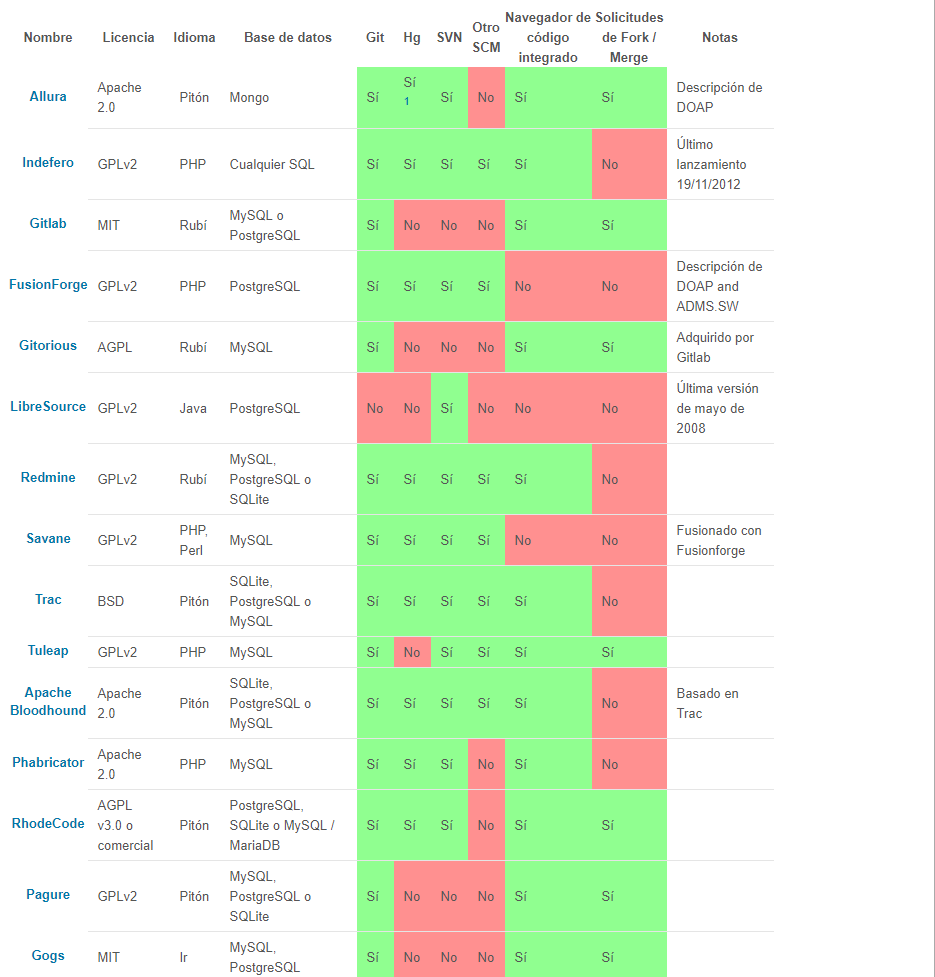
\includegraphics[width=17cm]{./Imagenes/cuadro1} 
	\end{center}

       


\end{itemize} 

\end{document}
